\input{text/diss}
\begin{document}
\def\labauthors{Виноградов И.Д., Шиков А.П.}
\def\labgroup{440}
\def\labnumber{1}
\def\labtheme{Исследование акустического поля в однородной среде с плоской границей}
\def\department{Кафедра акустики}
\newcommand{\D}[1]{D\qty[#1]}
\input{text/titlepage}

\paragraph{Цель работы:}

\section{Теоретическая часть}

\newpage
\section{Экспериментальная часть}
\paragraph{Описание установки}

\subsection{Диаграмма направленности излучателя}
Для снятия диаграммы направленности, излучатель был погружен в воду на глубину 15 см. Приемный щуп был расположен на той
же глубине, а расстояние от приемника определялось несколькими условиями.

Первое - проведение измерений в зоне Фраунгофера, для того, чтобы вести работу с сформировавшимся фронтом волны. Условие
выглядит следующим образом:
\begin{equation}
	L > \frac{2D^2}{\lambda} \Rightarrow L > \frac{2 \cdot 10^{-4}}{1.5 \cdot 10^{-3}} \simeq 0.13 \text{ м} 
	\label{eq:exp:fraungofer}
\end{equation}
где $L$ - расстояние между источником и приемником, $D$ - характерный размер источника(10 мм), $\lambda$ - длина волны
излучения ( $f = 1$ МГц, $\lambda = 1.5$ мм). 

Второе - прямой и отраженный импульс должны полностью разделяться по вермени прихода. Чтобы это условие выполнялось,
необходимо, чтобы время прихода отраженного импульса $t_2$ было больше, чем величина $t_1+\tau$, где $t_1$ - время
прихода прямого импульса, а $\tau$ - длительность импульса.
\begin{figure}[h!]
	\centering
	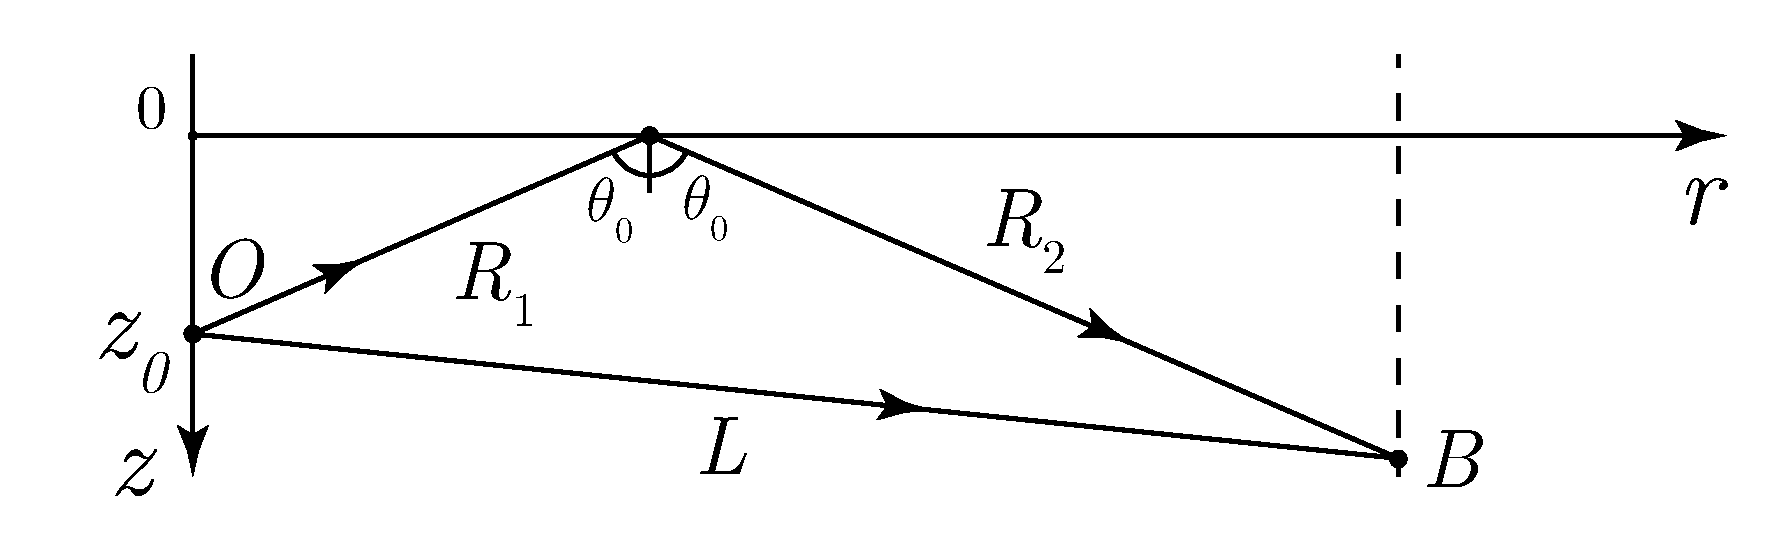
\includegraphics[width =0.7\linewidth]{fig/scheme2.pdf}
	\caption{Схема к рассчету расстояния меджу источником и приемником}
	\label{fig:expt:scheme2}
\end{figure}

\begin{equation}
	t_2 > t_1 + \tau, \quad t_1 = \frac{L}{c}, t_2 = \frac{R_1+R_2}{c}
\end{equation}
В достаточно грубом приближении, считая $L \sim 1$ м, а $R_1+R_2 \sim 1.5$ м, можно получить:
\begin{equation}
	\tau < \frac{R_1+R_2-L}{c} \simeq \frac{0.5}{1500} = 3 \cdot 10^{-4} \text{ с}
\end{equation}
\begin{equation}
	\tau < 300 \text{ мкс}
	\label{eq:time_cond}
\end{equation}
В работе использовалось $\tau = 100$ мкс, что удовлетворяет условию \eqref{eq:time_cond}.

Отнормированная диаграмма направленности излучателя, а также расчитанная теоретически в приближении плоского диска
приведены на рис. \ref{fig:direct}. В качестве теоретической характеристики использовалась характеристика круглой
плоской антенны с диаметром $d$:
\begin{equation}
	b(\theta) = \frac{2 J_1[ \frac{\pi d}{\lambda} \cos \theta ]}{\frac{\pi d}{\lambda} \cos \theta },
	\label{eq:bessel_disk}
\end{equation}
где $J_1$ - функция Бесселя первого порядка.
\begin{figure}[h!]
	\centering
	\includegraphics[width=0.9\linewidth]{fig/direct.png}
	\caption{Нормированная диаграммма направленности излучателя, и теоретическая характеристика для плоского диска}
	\label{fig:direct}
\end{figure}

\subsection{Исследование распределения звукового давления}
\begin{figure}[h!]
	\centering
	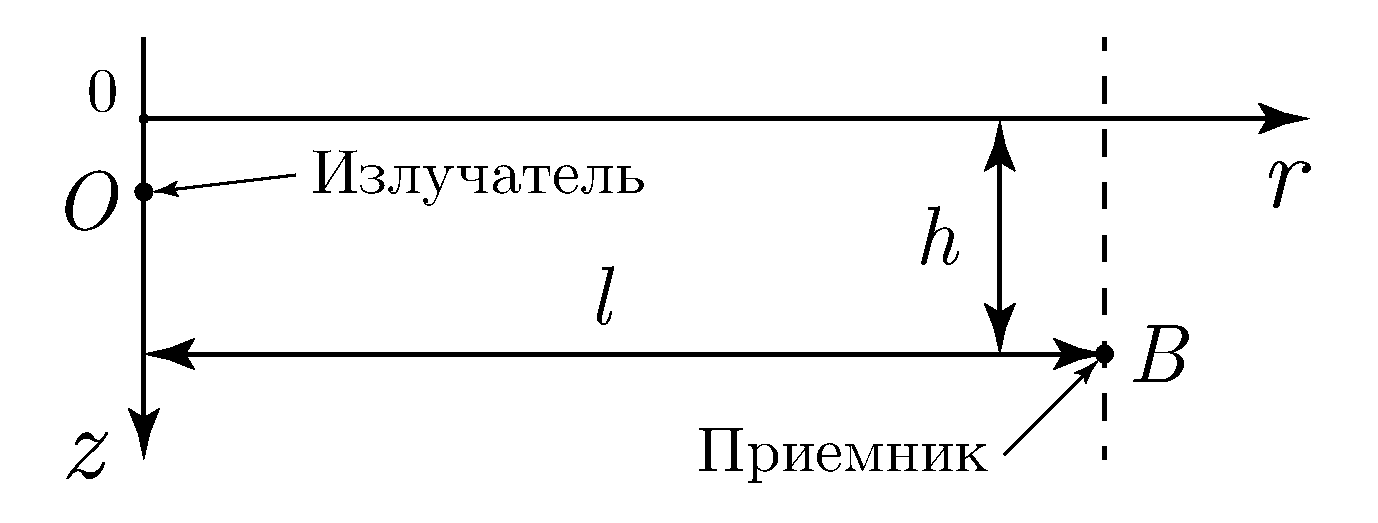
\includegraphics[width =0.6\linewidth]{fig/scheme3.pdf}
	\caption{Схема постановки эксперимента}
	\label{fig:expt:scheme3}
\end{figure}
Излучатель был расположен на глубине $\sim 2.5$ см, чтобы полностью быть погруженным в воду.
С помощью приемного щупа было произведено исследовано распределение звукового давления в ванне, были произведены три
продольных разреза на глубинах $h = 1,2.5,4$ см, и три вертикальных среза на расстояниях $l=70,100,130$ см.

Теоретическое значение для модуля амплитуды суммарного давления рассчитывалось по формуле \eqref{eq:pressure}:
\begin{equation}
	|P(h,R)| = \sqrt{ \frac{1}{R^2} + \frac{1}{R_1^2} - \frac{2}{R_1 R} \cos k \Delta R },\quad \Delta R = R-R_1,
	\label{eq:pressure}
\end{equation}
где $R^2 = l^2+(h-z_0)^2$, а $R_1^2 = l^2 + (h+z_0)^2$, $k$ - волновое число.

\begin{figure}[h!]
	\centering
	\includegraphics[width =0.75\linewidth]{fig/task21}
	\caption{Амплитуды максимумов и минимумов при продольном срезе, на глубине $h=1$ см}
	\label{fig:task21}
\end{figure}

\begin{figure}[h!]
	\centering
	\includegraphics[width =0.75\linewidth]{fig/task22}
	\caption{Амплитуды максимумов и минимумов при продольном срезе, на глубине $h=2.5$ см}
	\label{fig:task22}
\end{figure}

\begin{figure}[h!]
	\centering
	\includegraphics[width =0.75\linewidth]{fig/task23}
	\caption{Амплитуды максимумов и минимумов при продольном срезе, на глубине $h=4$ см}
	\label{fig:task23}
\end{figure}

\end{document}
